% latex table generated in R 3.6.3 by xtable 1.8-4 package
% Thu Jan 18 11:33:54 2024
\begin{table}[ht]
\centering
\begin{tabular}{rlrrr}
  \hline
 & OTU & MeanRA & MedianRA & SE \\ 
  \hline
419610 & Methylorubrum extorquens & 0.00006533 & 0.00005353 & 0.00001571 \\ 
  32009 & Burkholderia gladioli & 0.00004414 & 0.00004435 & 0.00000339 \\ 
  640081 & Azospira oryzae & 0.00006336 & 0.00005796 & 0.00000936 \\ 
  2706126 & Pseudomonas sp. OIL- & 0.00005744 & 0.00005843 & 0.00000328 \\ 
  2726989 & Pseudomonas sp. gcc2 & 0.00005071 & 0.00004922 & 0.00000329 \\ 
  76760 & Pseudomonas rhodesia & 0.00004632 & 0.00004114 & 0.00000576 \\ 
  553151 & Halopseudomonas pelagi & 0.00005750 & 0.00006352 & 0.00000567 \\ 
  219572 & Pseudomonas antarctic & 0.00004038 & 0.00003570 & 0.00000376 \\ 
  163011 & Pseudomonas lin & 0.00004752 & 0.00003619 & 0.00001561 \\ 
  64187 & Xanthomonas oryzae & 0.00004090 & 0.00003884 & 0.00000303 \\ 
  349967 & Yersinia mollaretii & 0.00000693 & 0.00000691 & 0.00000067 \\ 
  213554 & Halomonas campaniensi & 0.00000240 & 0.00000200 & 0.00000086 \\ 
  28084 & Legionella cherri & 0.00000718 & 0.00000570 & 0.00000212 \\ 
  92644 & Streptomyces malaysiensi & 0.00003218 & 0.00003575 & 0.00000554 \\ 
  67260 & Streptomyces cinereorube & 0.00002301 & 0.00002338 & 0.00000287 \\ 
  556325 & Neomicrococcus aestuari & 0.00003666 & 0.00003595 & 0.00000502 \\ 
  1520670 & [Mycobacterium] stephanolepidi & 0.00004888 & 0.00004736 & 0.00000707 \\ 
  33035 & Blautia product & 0.00001165 & 0.00001107 & 0.00000076 \\ 
  2214 & Methanosarcina acetivoran & 0.00000506 & 0.00000397 & 0.00000123 \\ 
  1903276 & Candidatus Nitrosotalea okcheonensi & 0.00001042 & 0.00000944 & 0.00000316 \\ 
  1410606 & Candidatus Nitrosopelagicus brevi & 0.00000579 & 0.00000431 & 0.00000191 \\ 
  2271 & Thermoproteus tena & 0.00000577 & 0.00000552 & 0.00000157 \\ 
   \hline
\end{tabular}
\caption{Keystone OTUs of } 
\end{table}
\begin{figure}
\centering
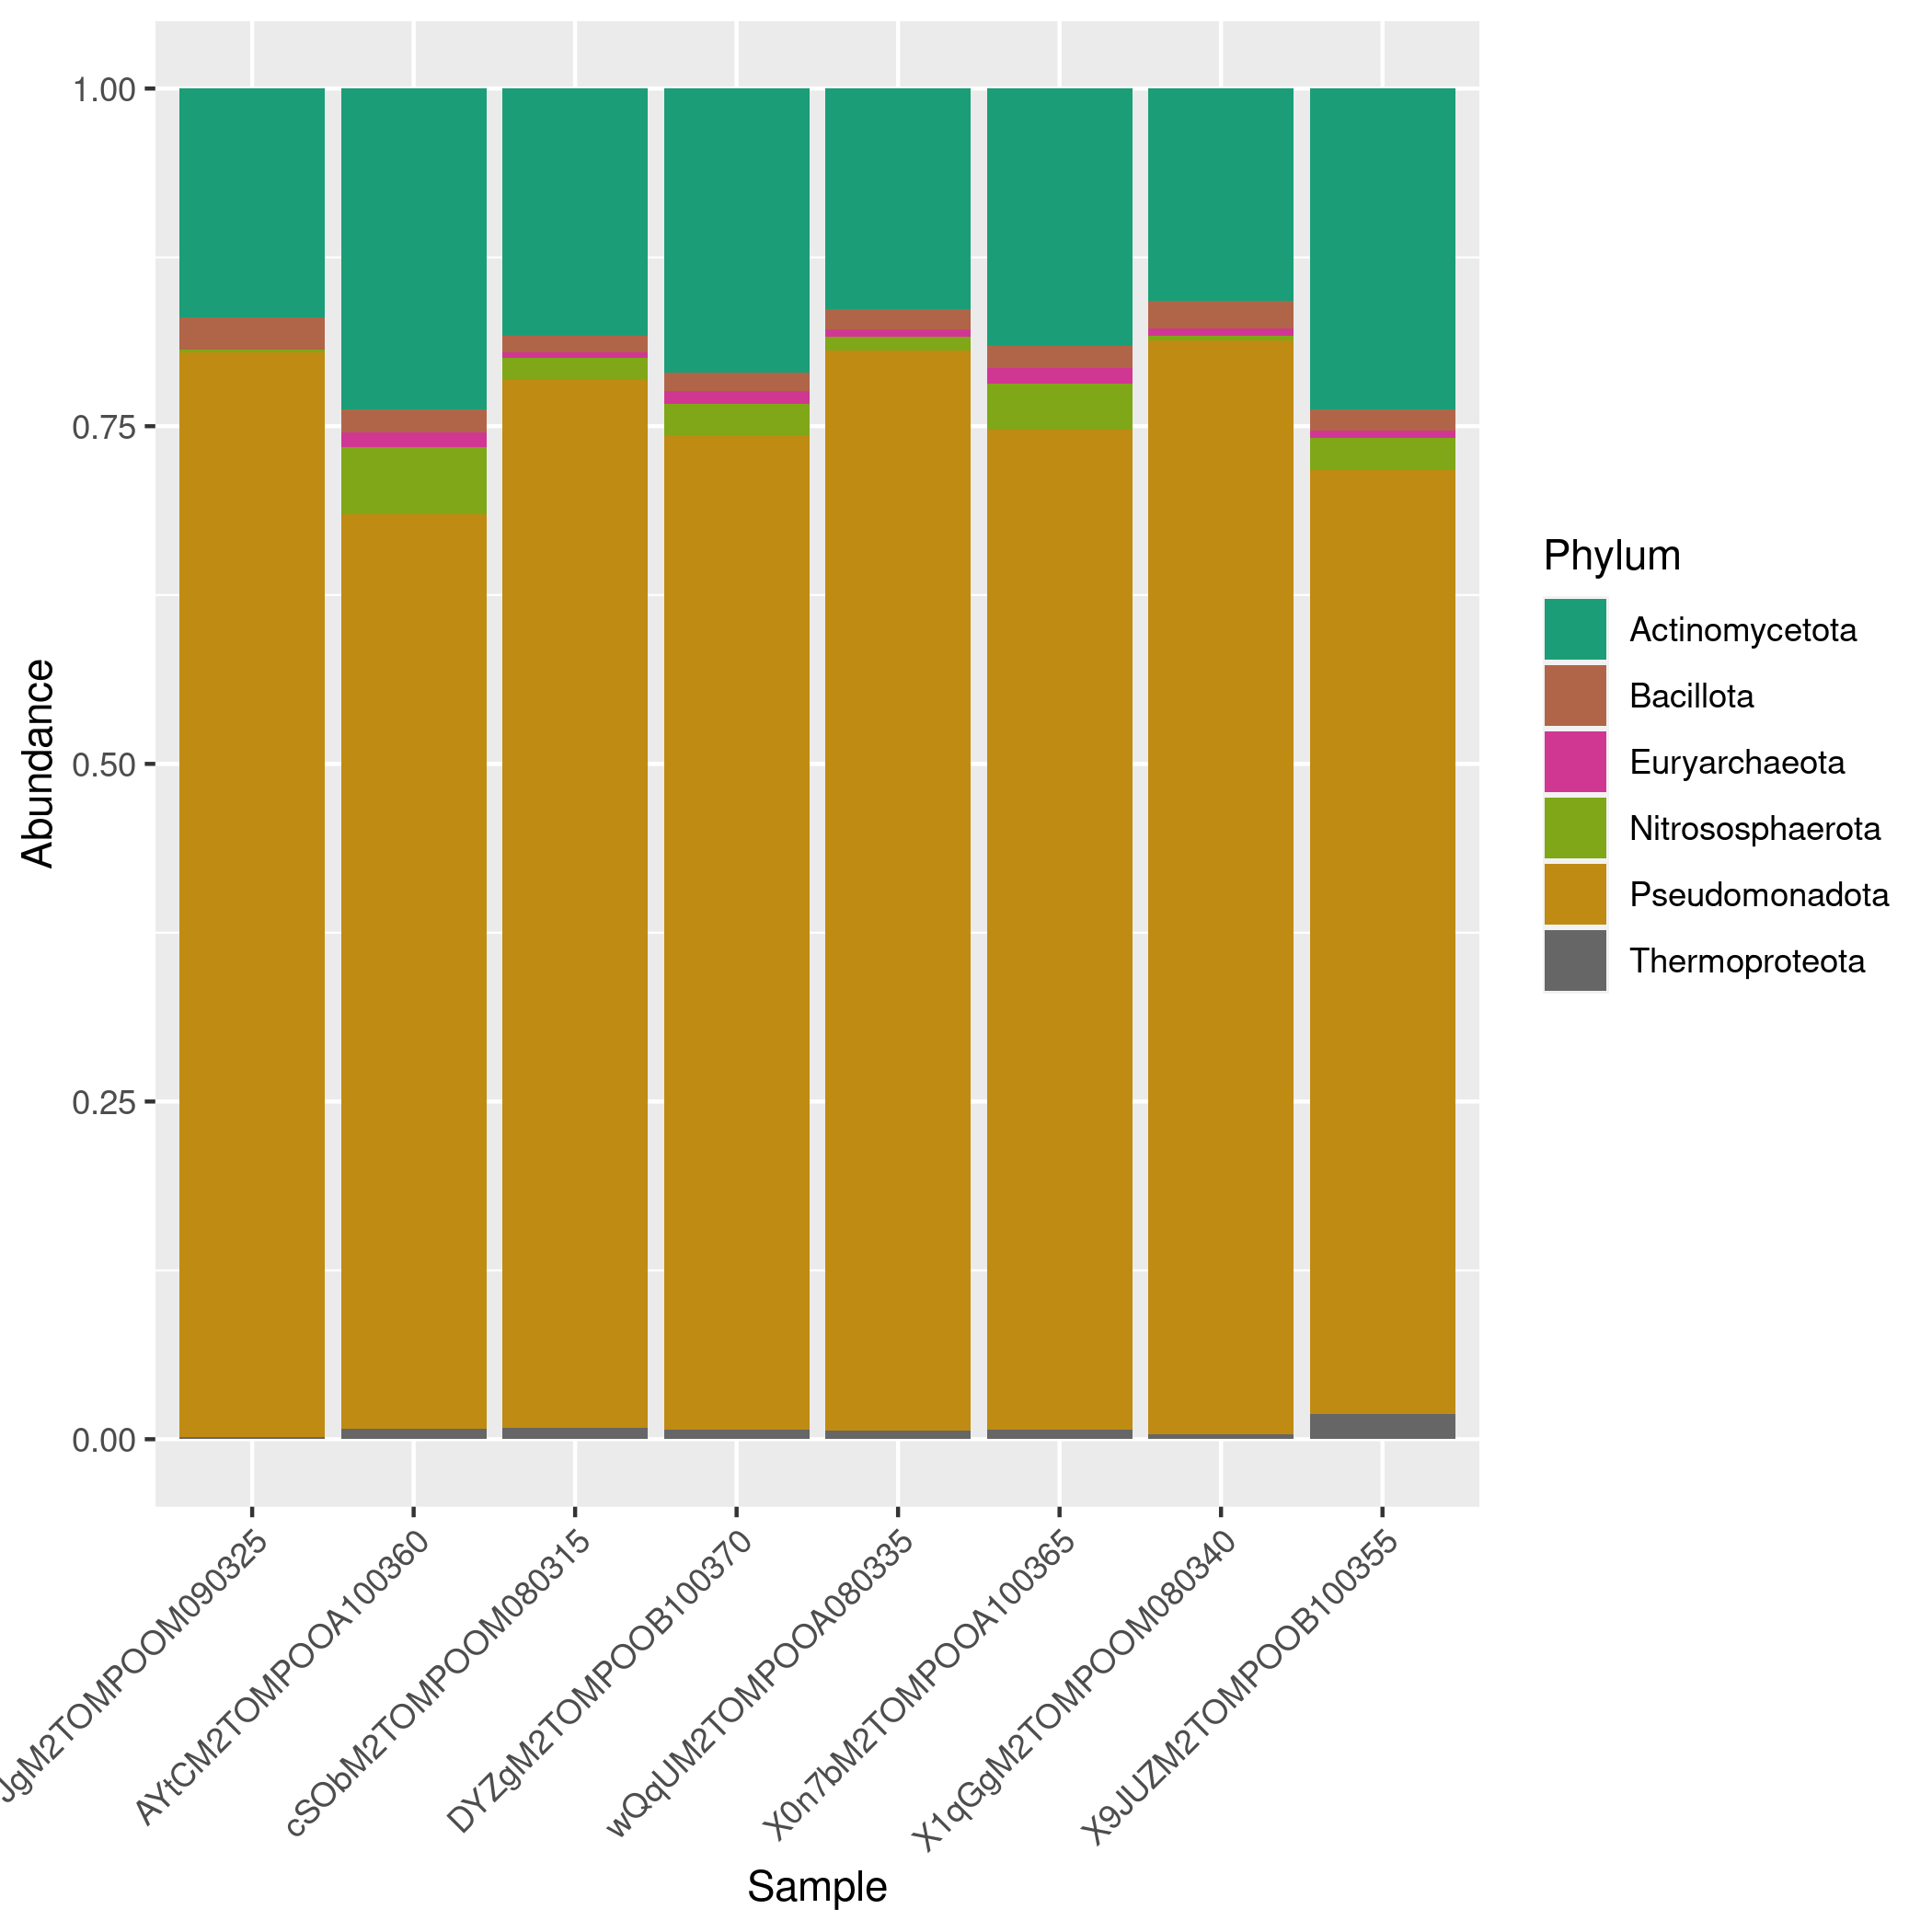
\includegraphics[scale = 0.8]{tomate_no_desarrollo.csv_relative_abundance_Phylum.png}
\caption{Relative abundance by phyla of keystone OTUs }
\label{fig:tomate_no_desarrollo.csv_phyla}
\end{figure}
\begin{figure}
\centering
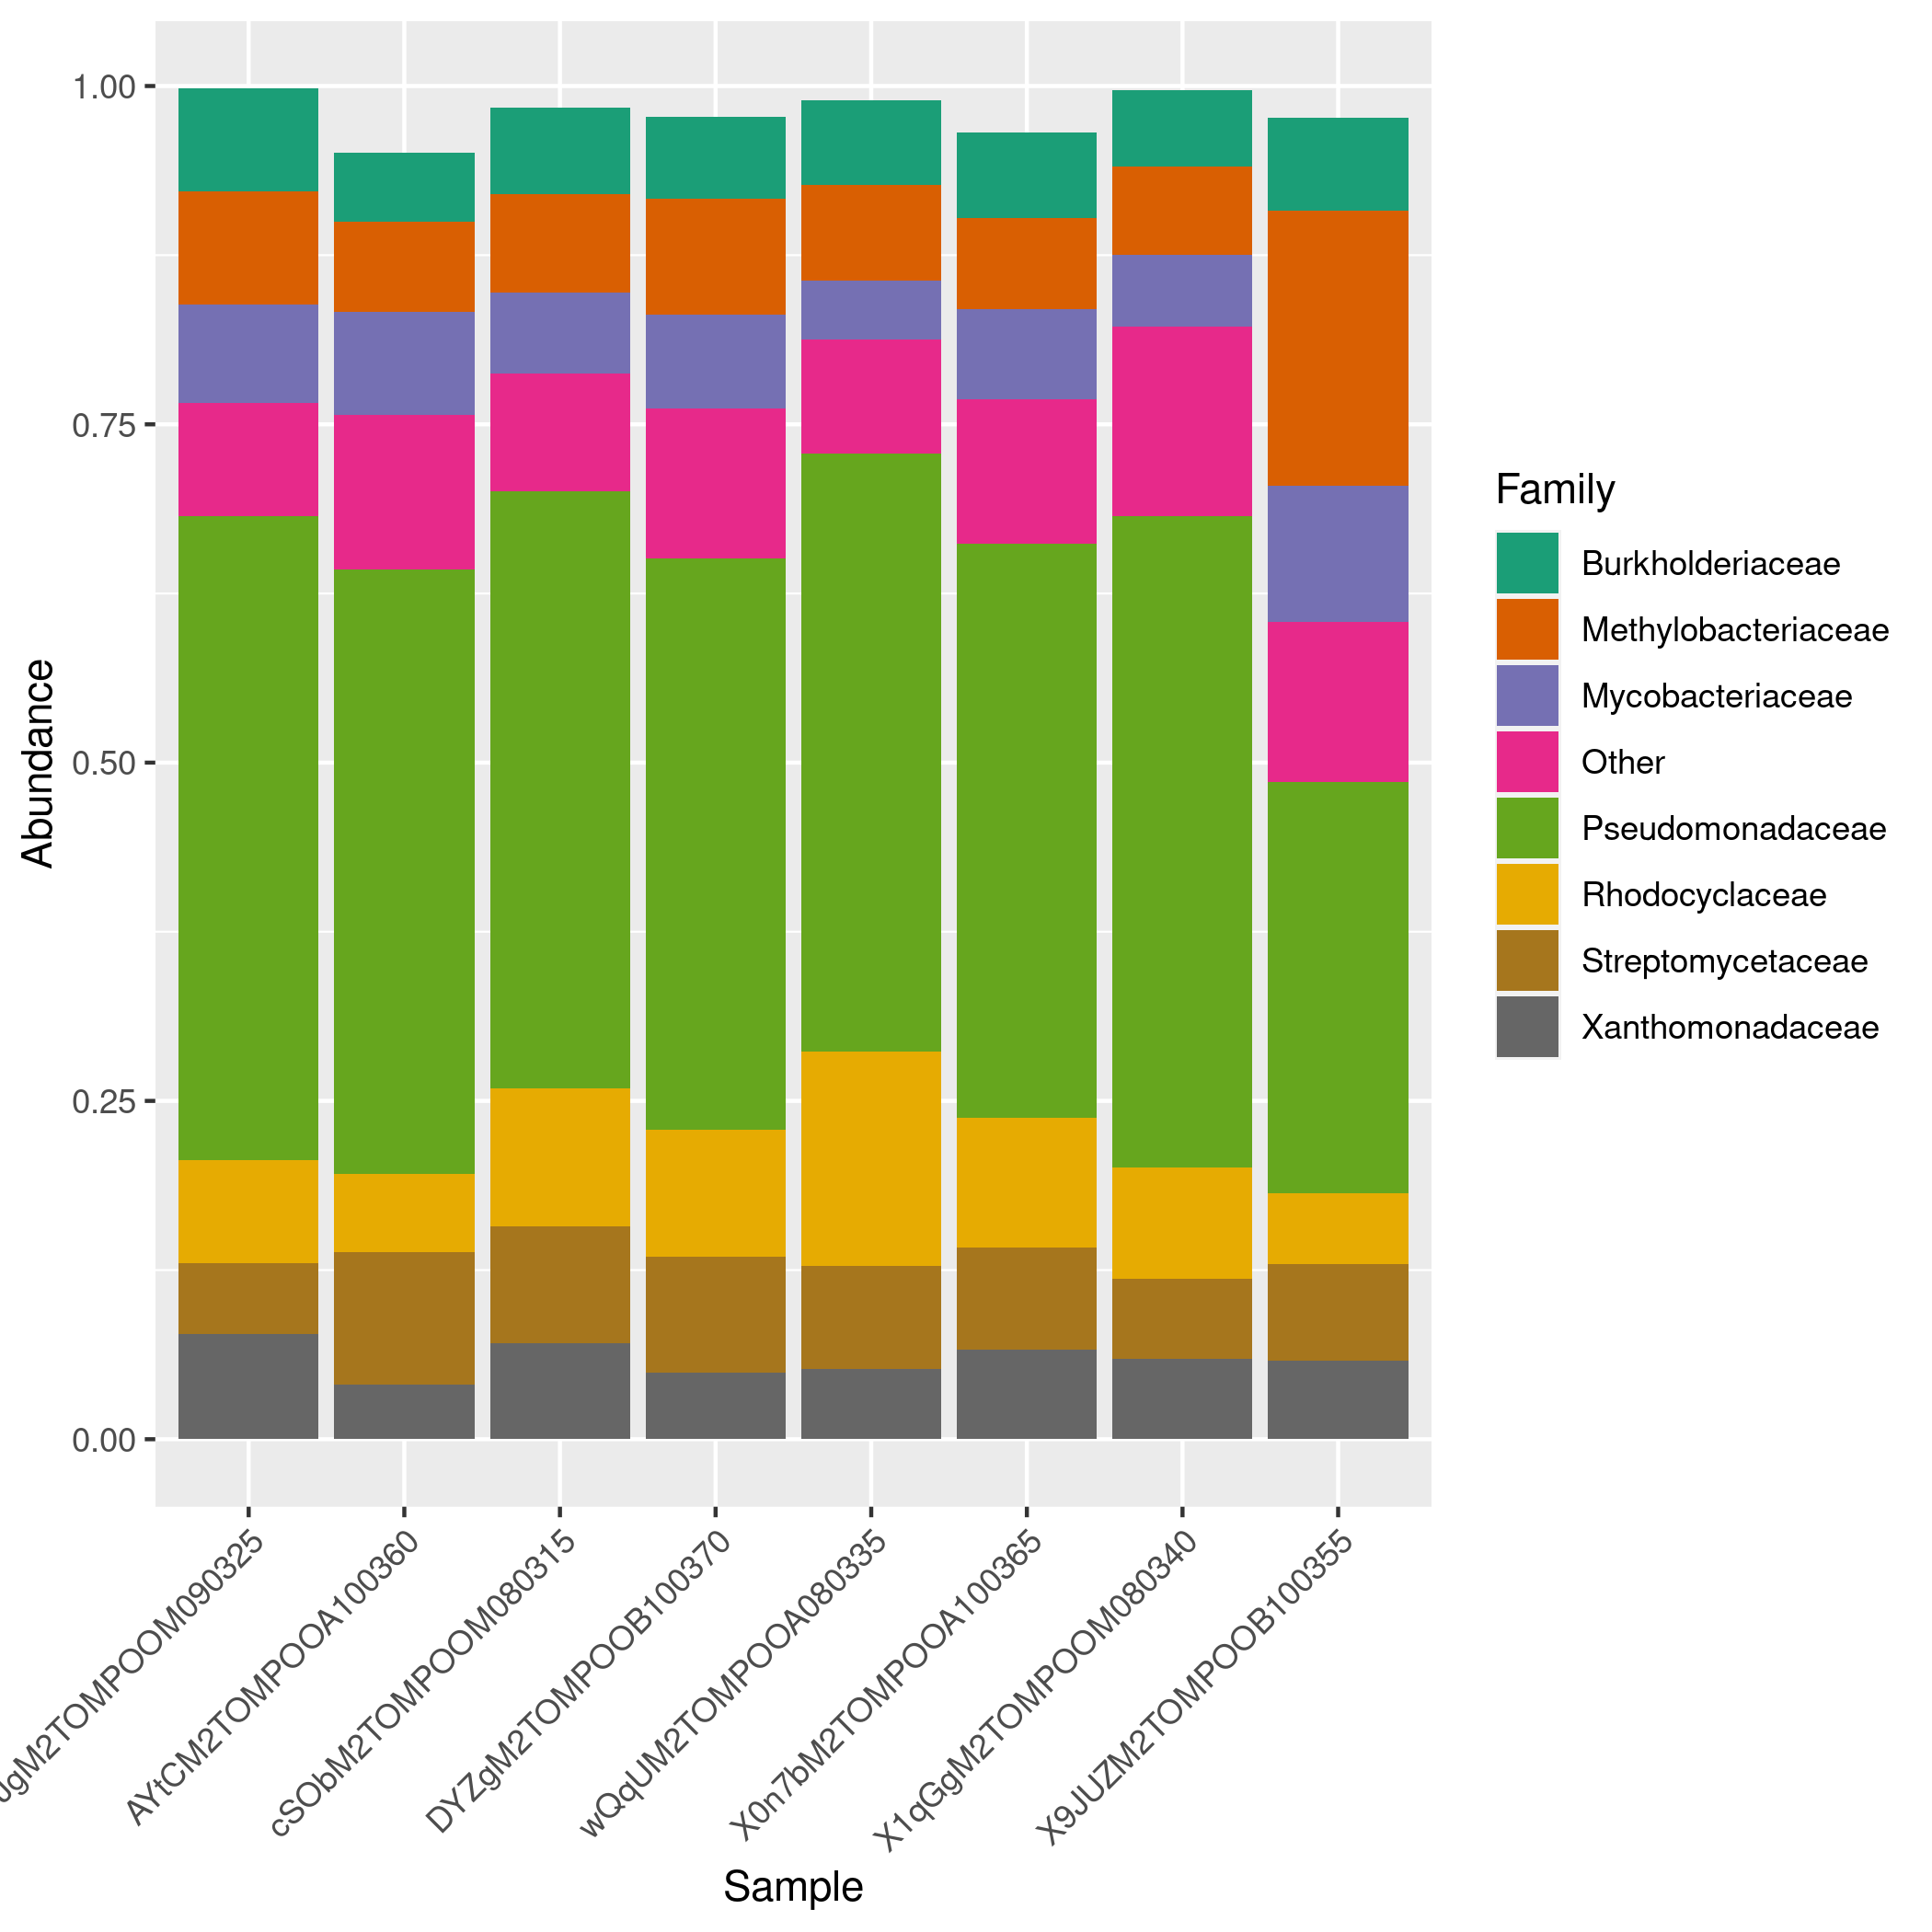
\includegraphics[scale = 0.8]{tomate_no_desarrollo.csv_relative_abundance_Family.png}
\caption{Relative abundance by families of keystone OTUs }
\label{fig:tomate_no_desarrollo.csv_family}
\end{figure}
\begin{figure}
\centering
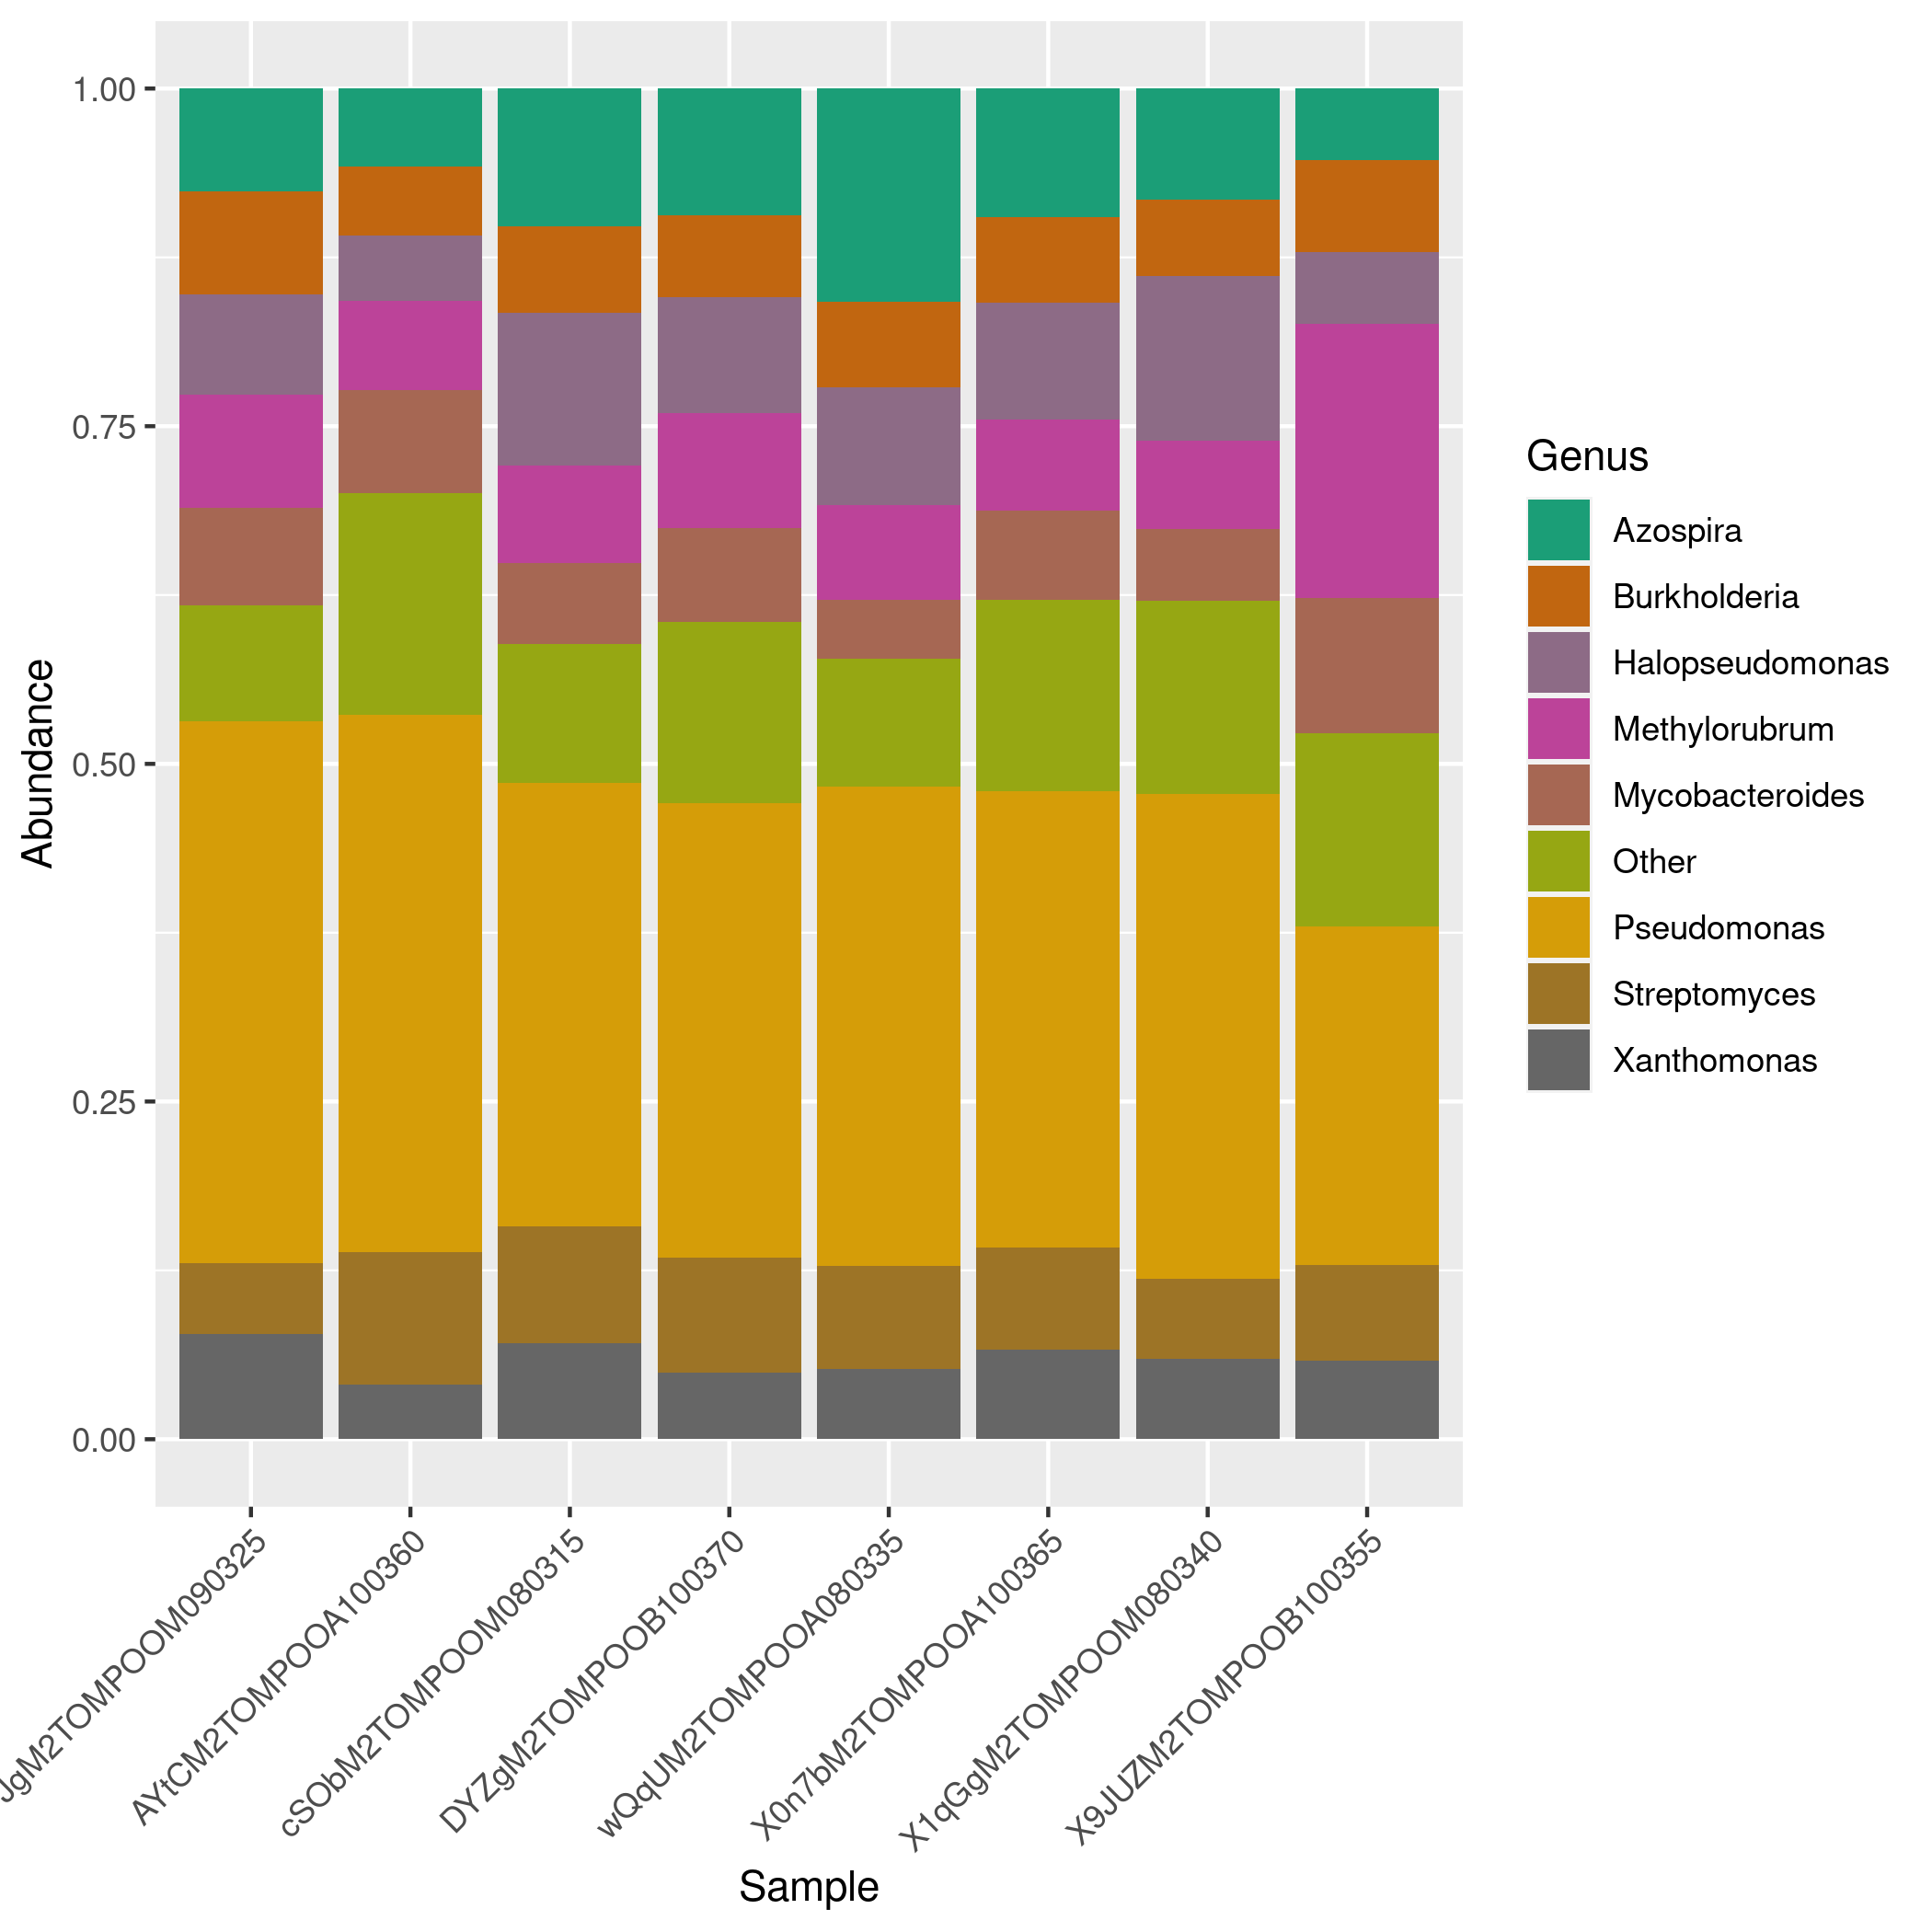
\includegraphics[scale = 0.8]{tomate_no_desarrollo.csv_relative_abundance_Genus.png}
\caption{Relative abundance by genera of keystone OTUs }
\label{fig:tomate_no_desarrollo.csv_genus}
\end{figure}
\begin{figure}
   \centering
   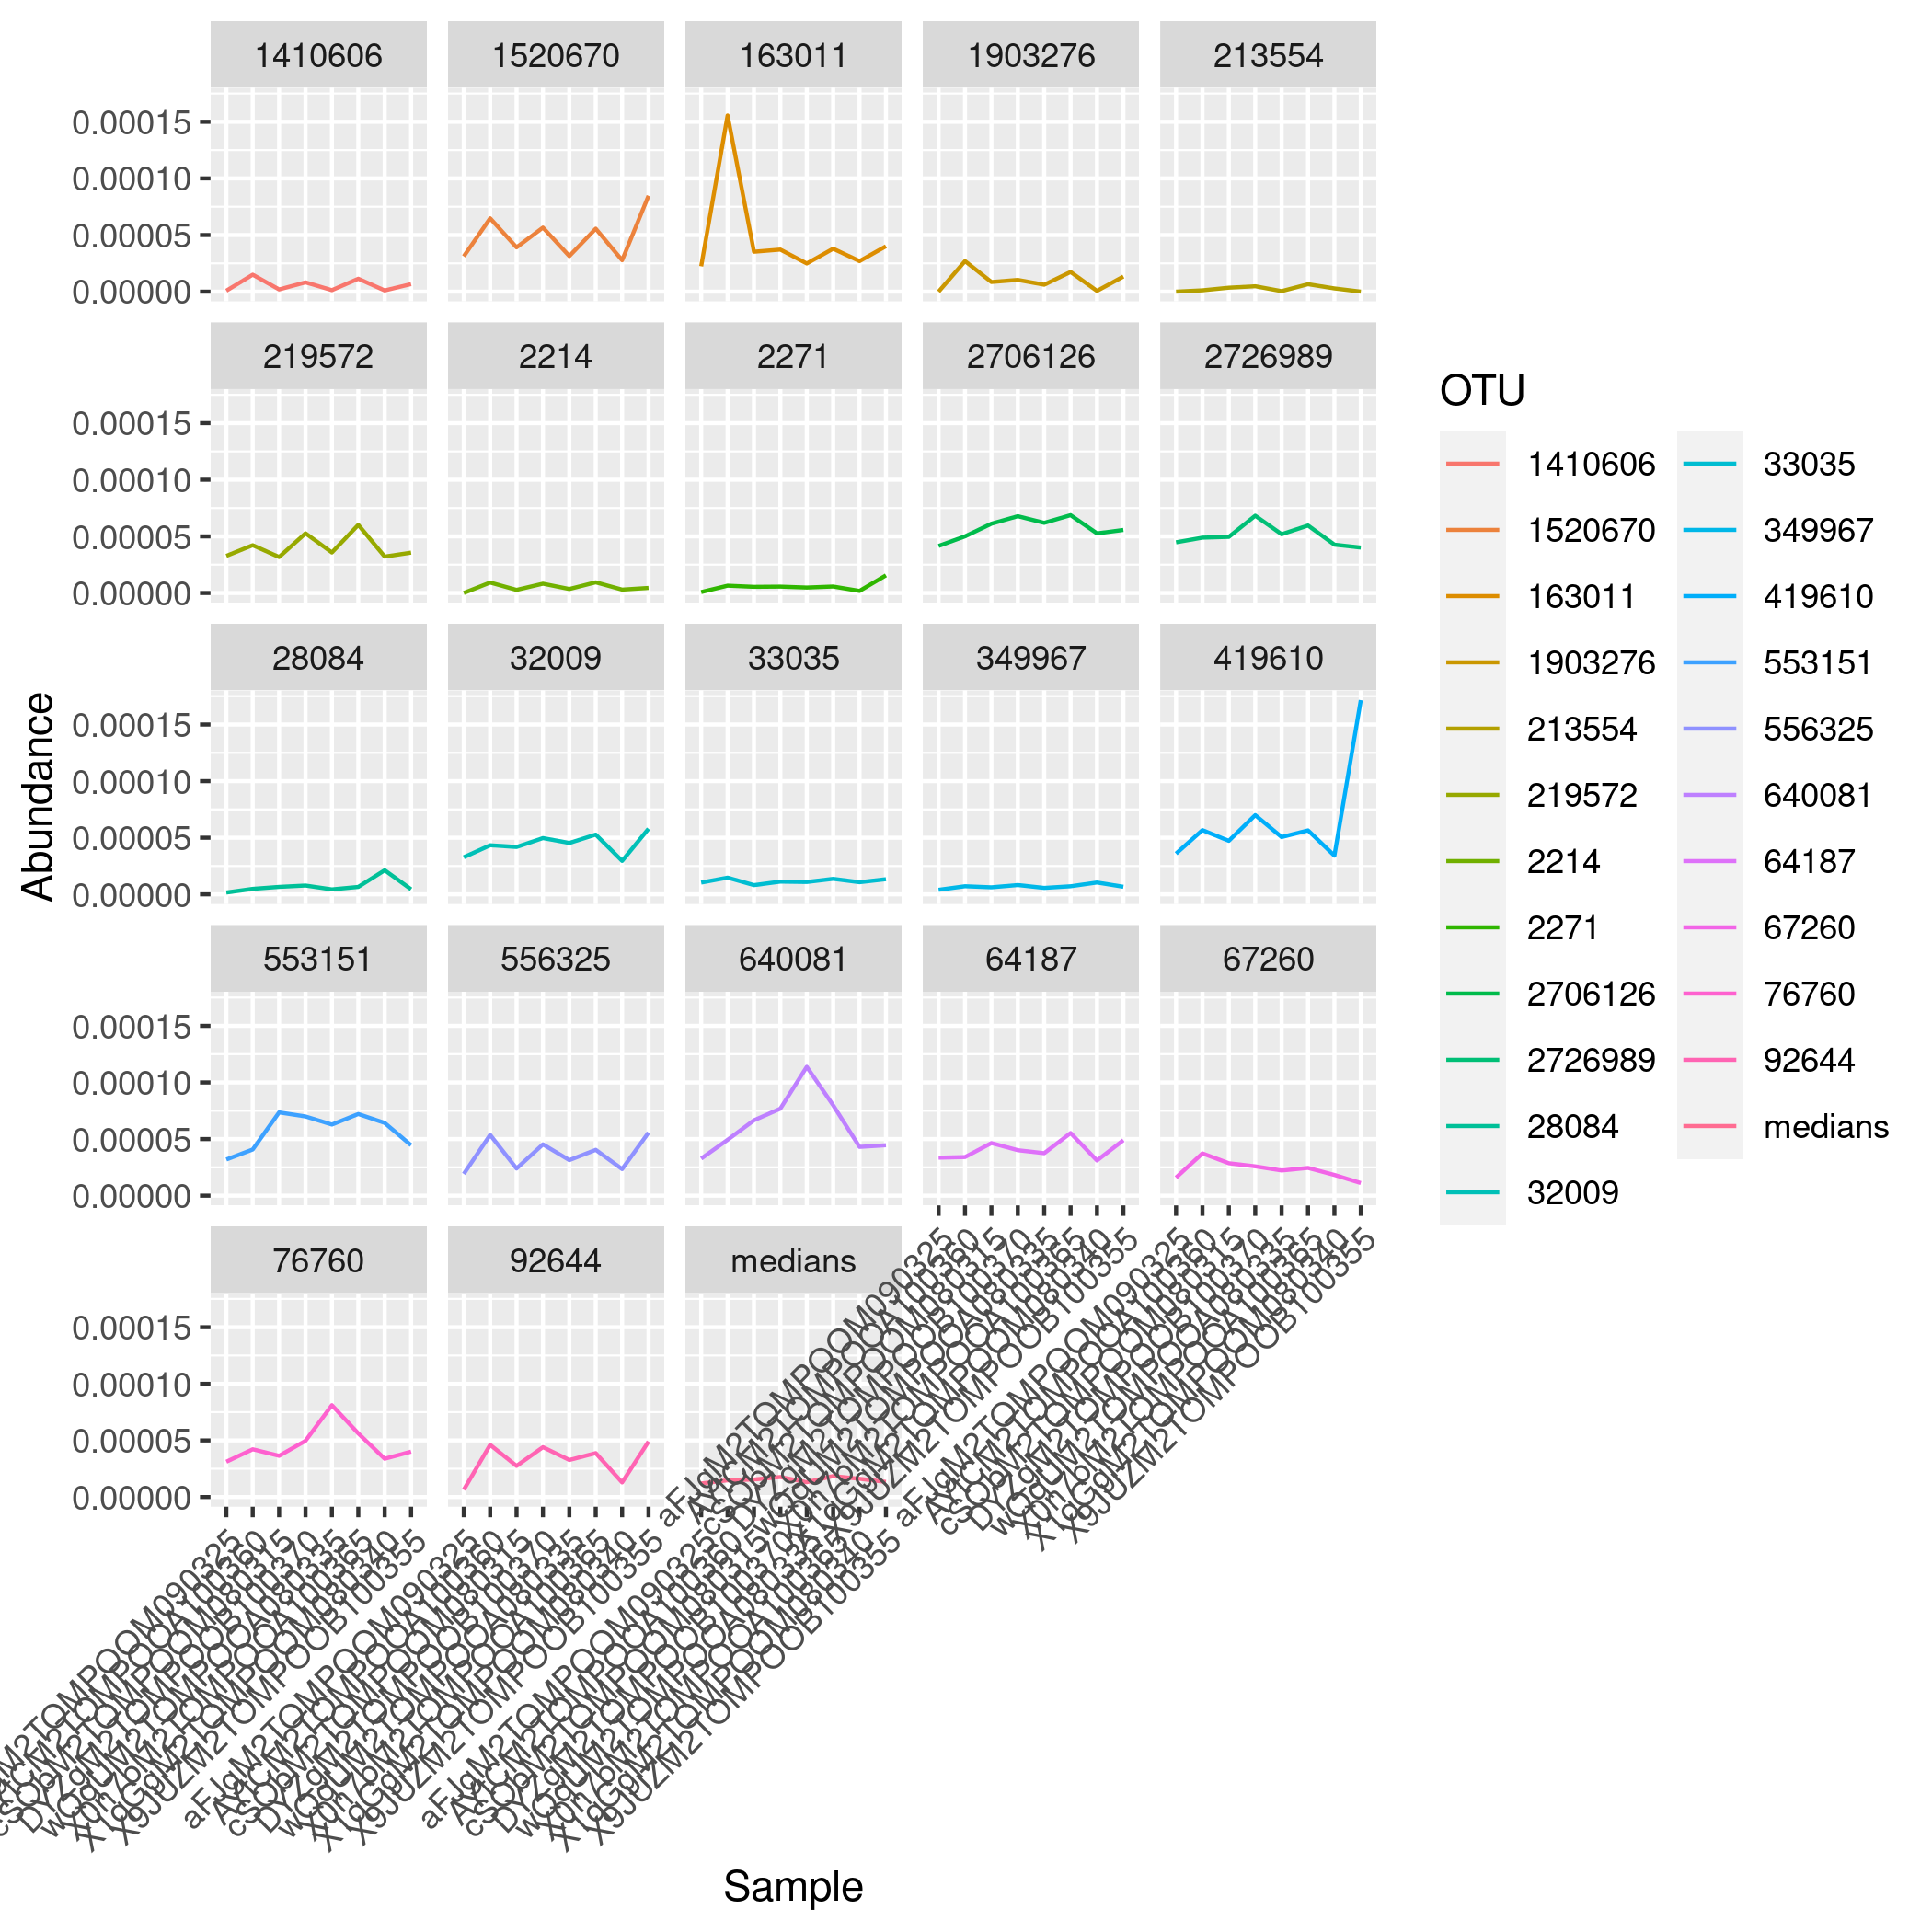
\includegraphics[scale = 0.8]{abundance_tomate_no_desarrollo.csv_key_otus_medians.png}
   \caption{Plots representing relative abundance of each keystone OTU and one representing the median relative abundance  across samples of rhizosphere of tomate_no_desarrollo.csv. Most keystone OTUs have relative abundance bigger than the median across all samples.  }
   \label{key_otus_vs_medians_tomate_no_desarrollo.csv}
\end{figure}
\begin{figure}
 \centering
 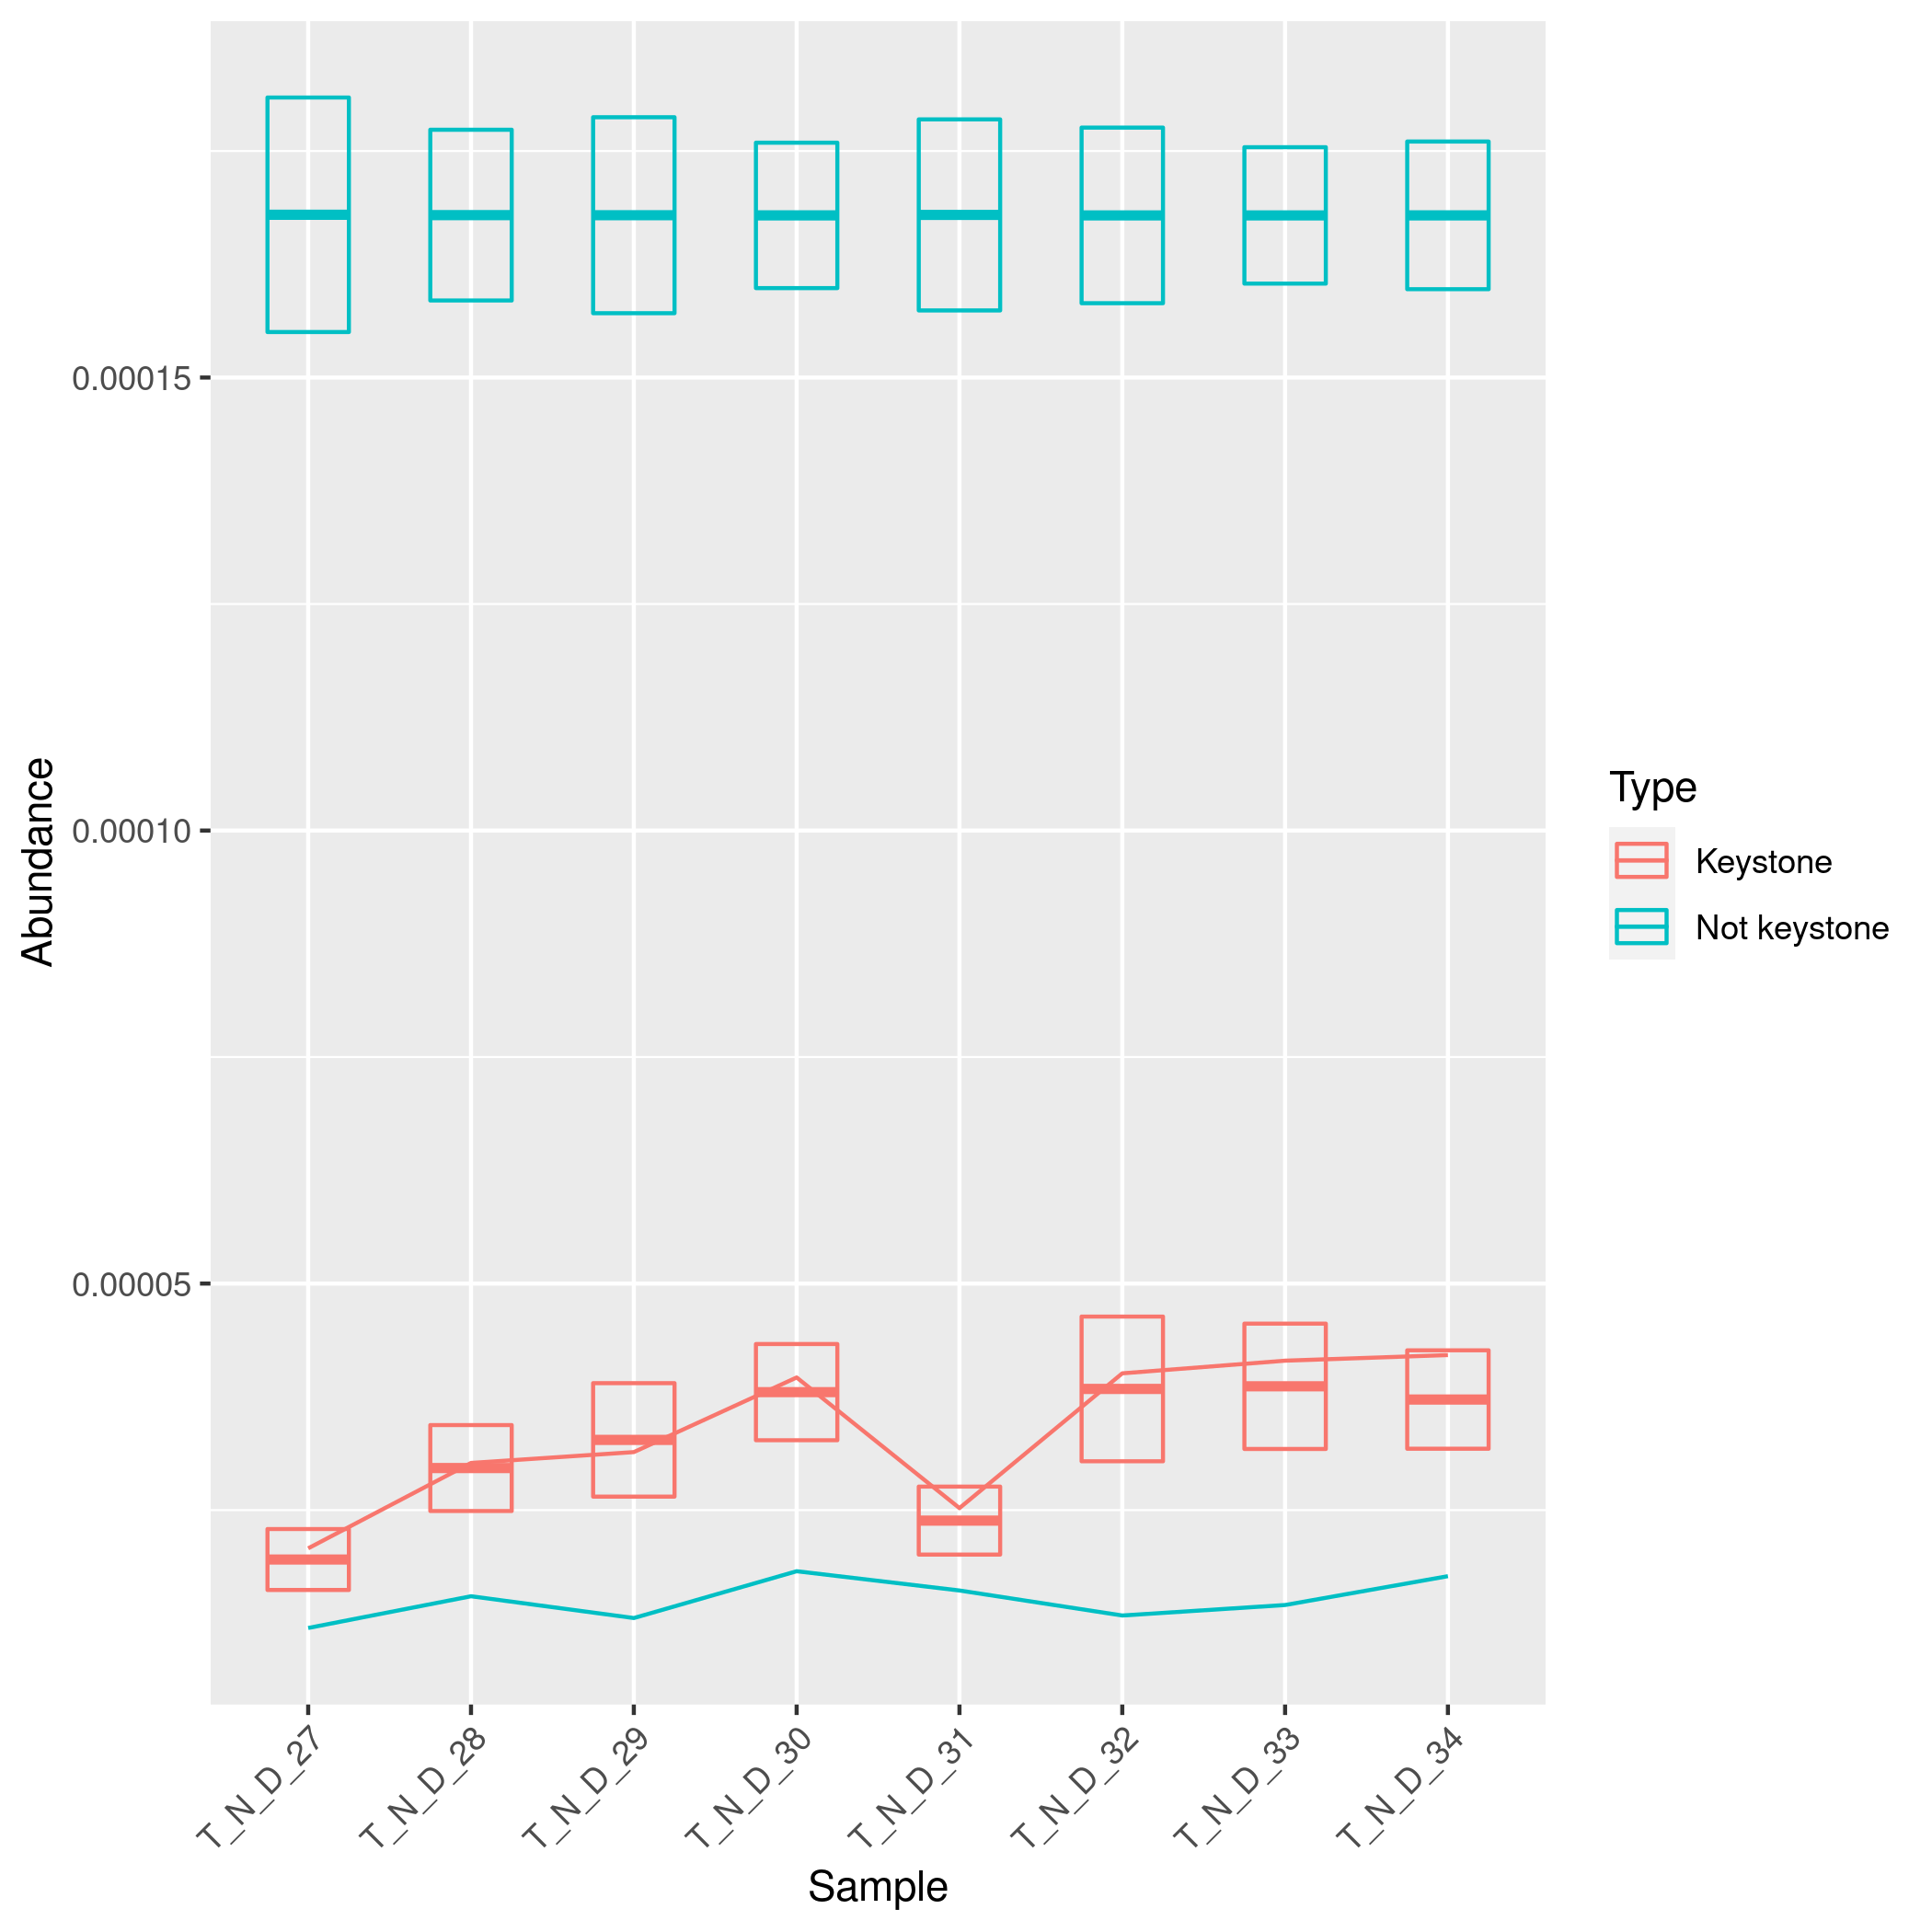
\includegraphics[scale = 0.75]{mean_median_key_vs_not_key_tomate_no_desarrollo.csv.png}
\caption{Boxes represent mean and standard error in the distribution of corresponding samples. Lines represent the corresponding medians. In these samples of rhizosphere oftomate_no_desarrollo.csv}
\label{mean_median_tomate_no_desarrollo.csv}
\end{figure}
\begin{figure}
   \centering
   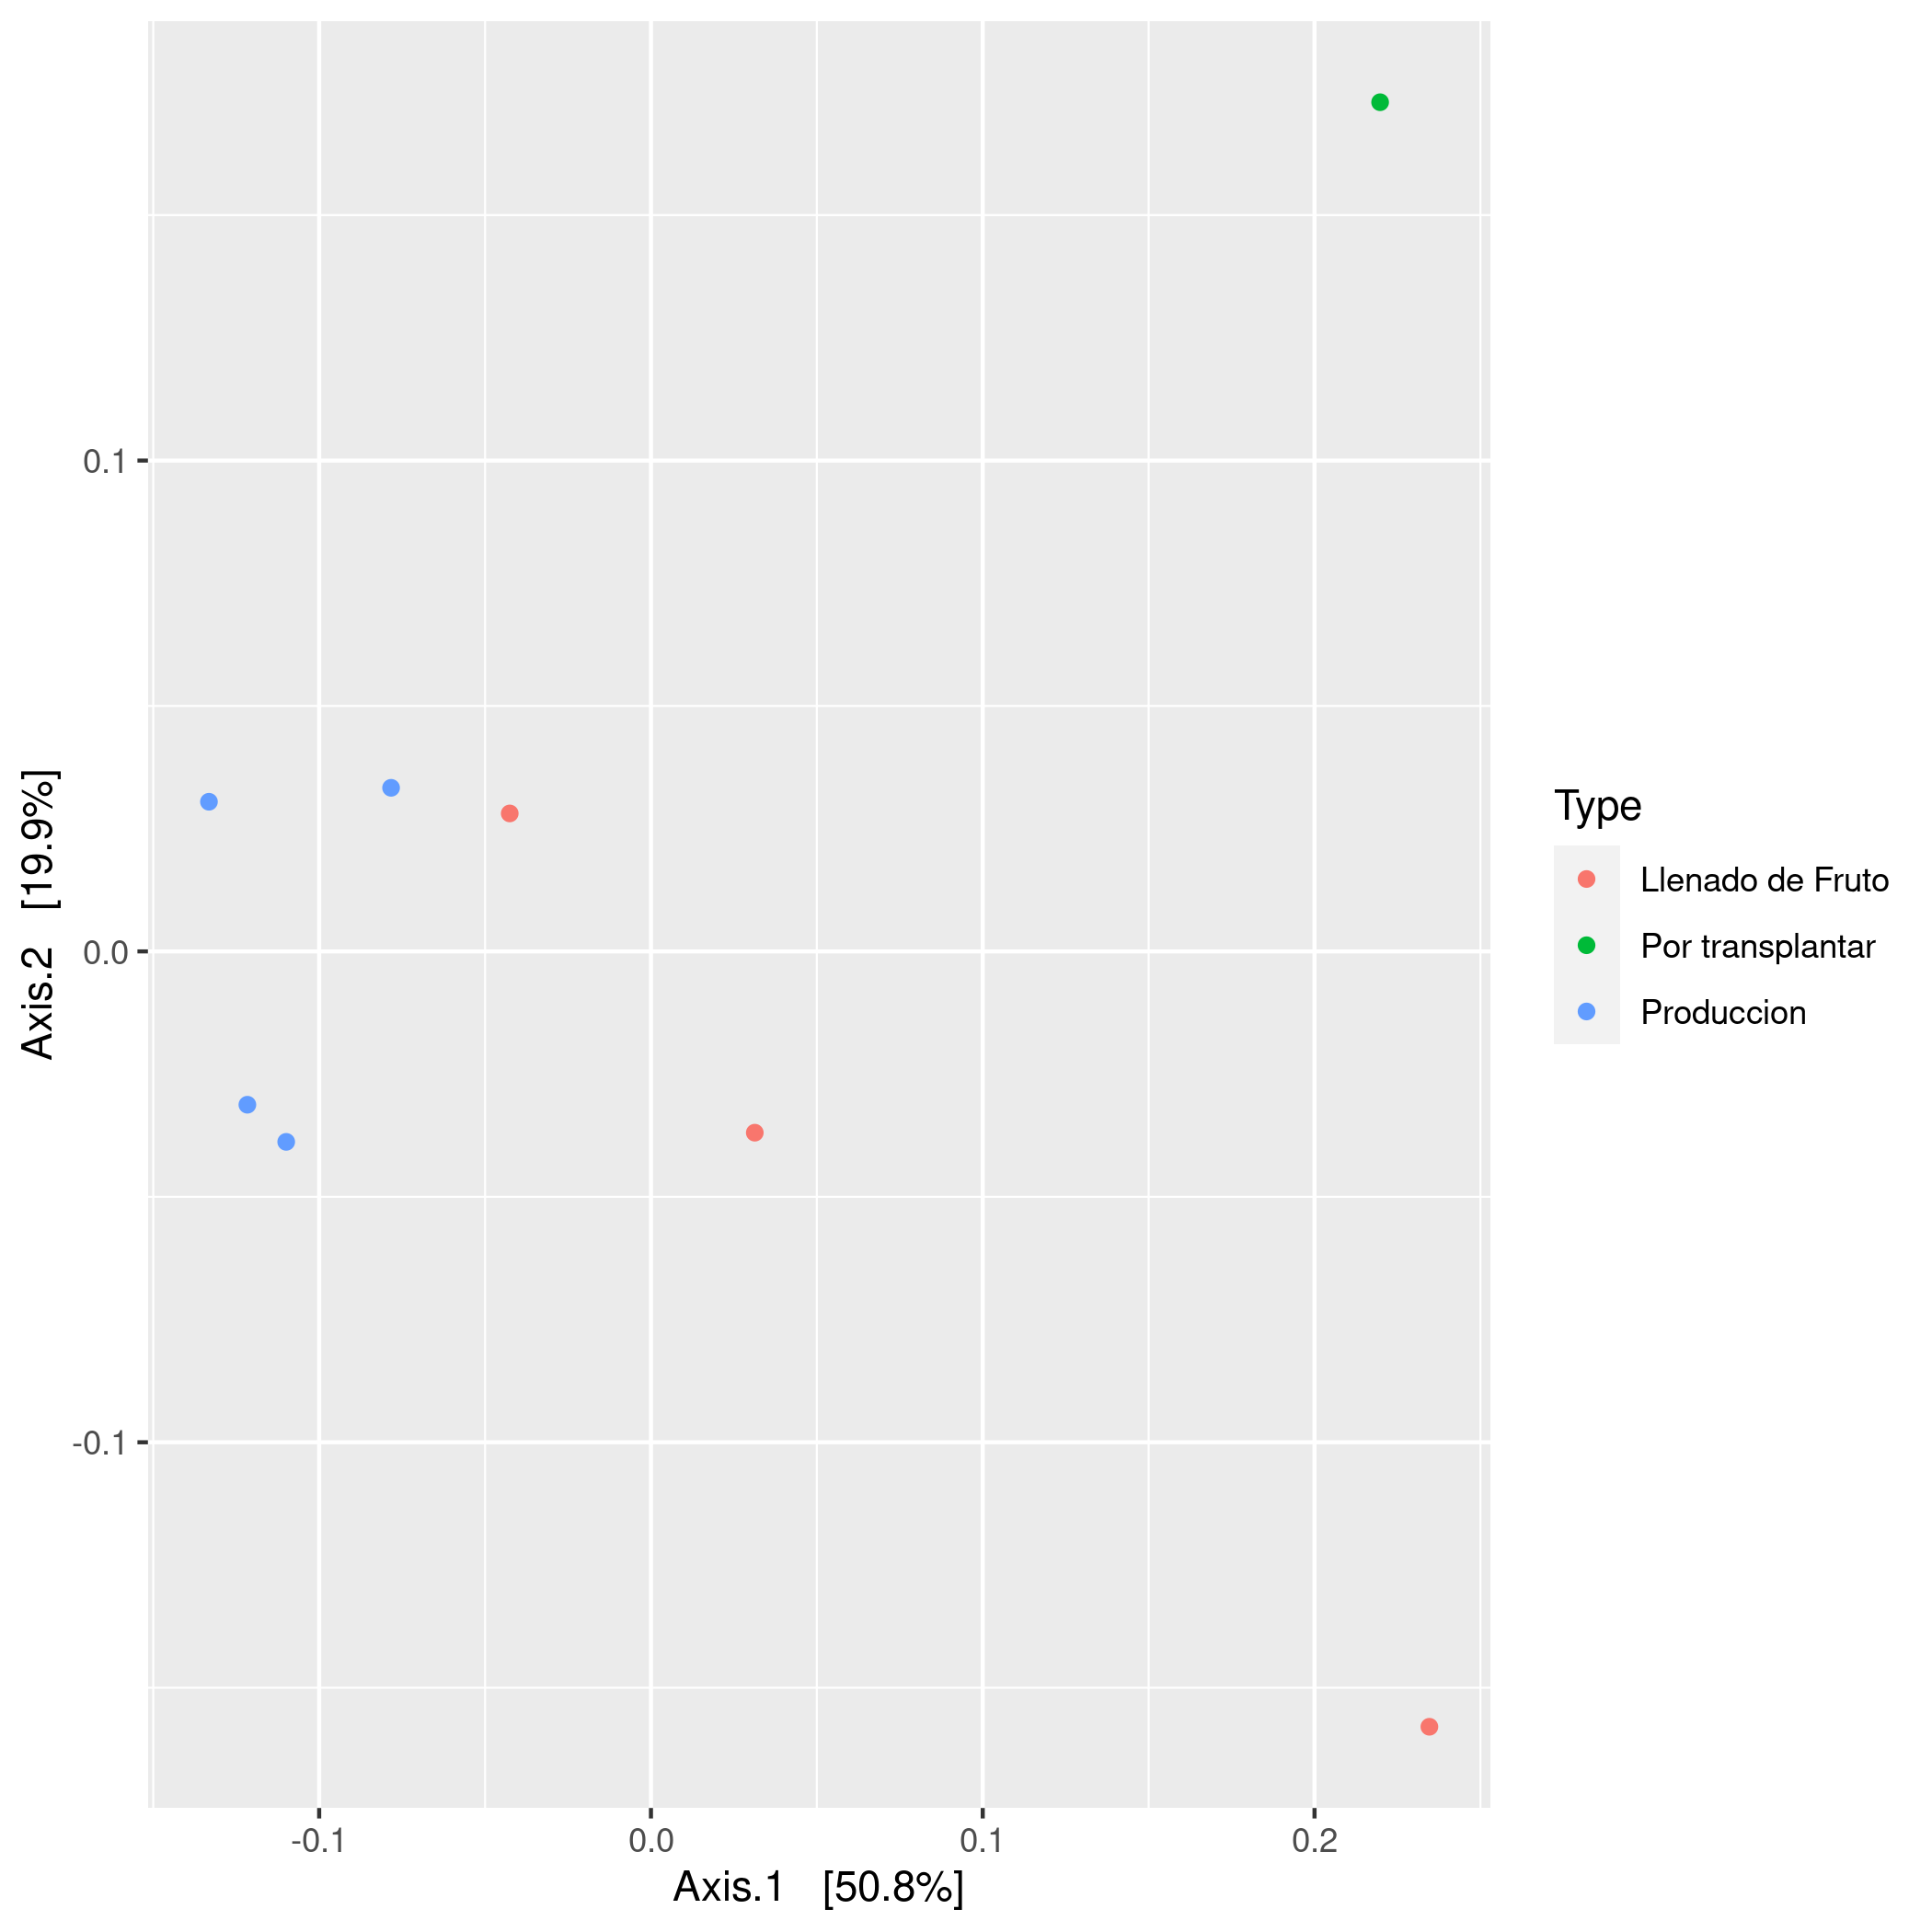
\includegraphics[scale = 0.7]{pcoa_muestras_tomate_no_desarrollo.csv.png}
 \caption{PCoA analysis with Bray-Curtis distance of rhizosphere samples of tomate_no_desarrollo.csv.}
 \label{fig:tomate_no_desarrollo.csv_pcoa}
\end{figure}
\begin{figure}
  \centering
  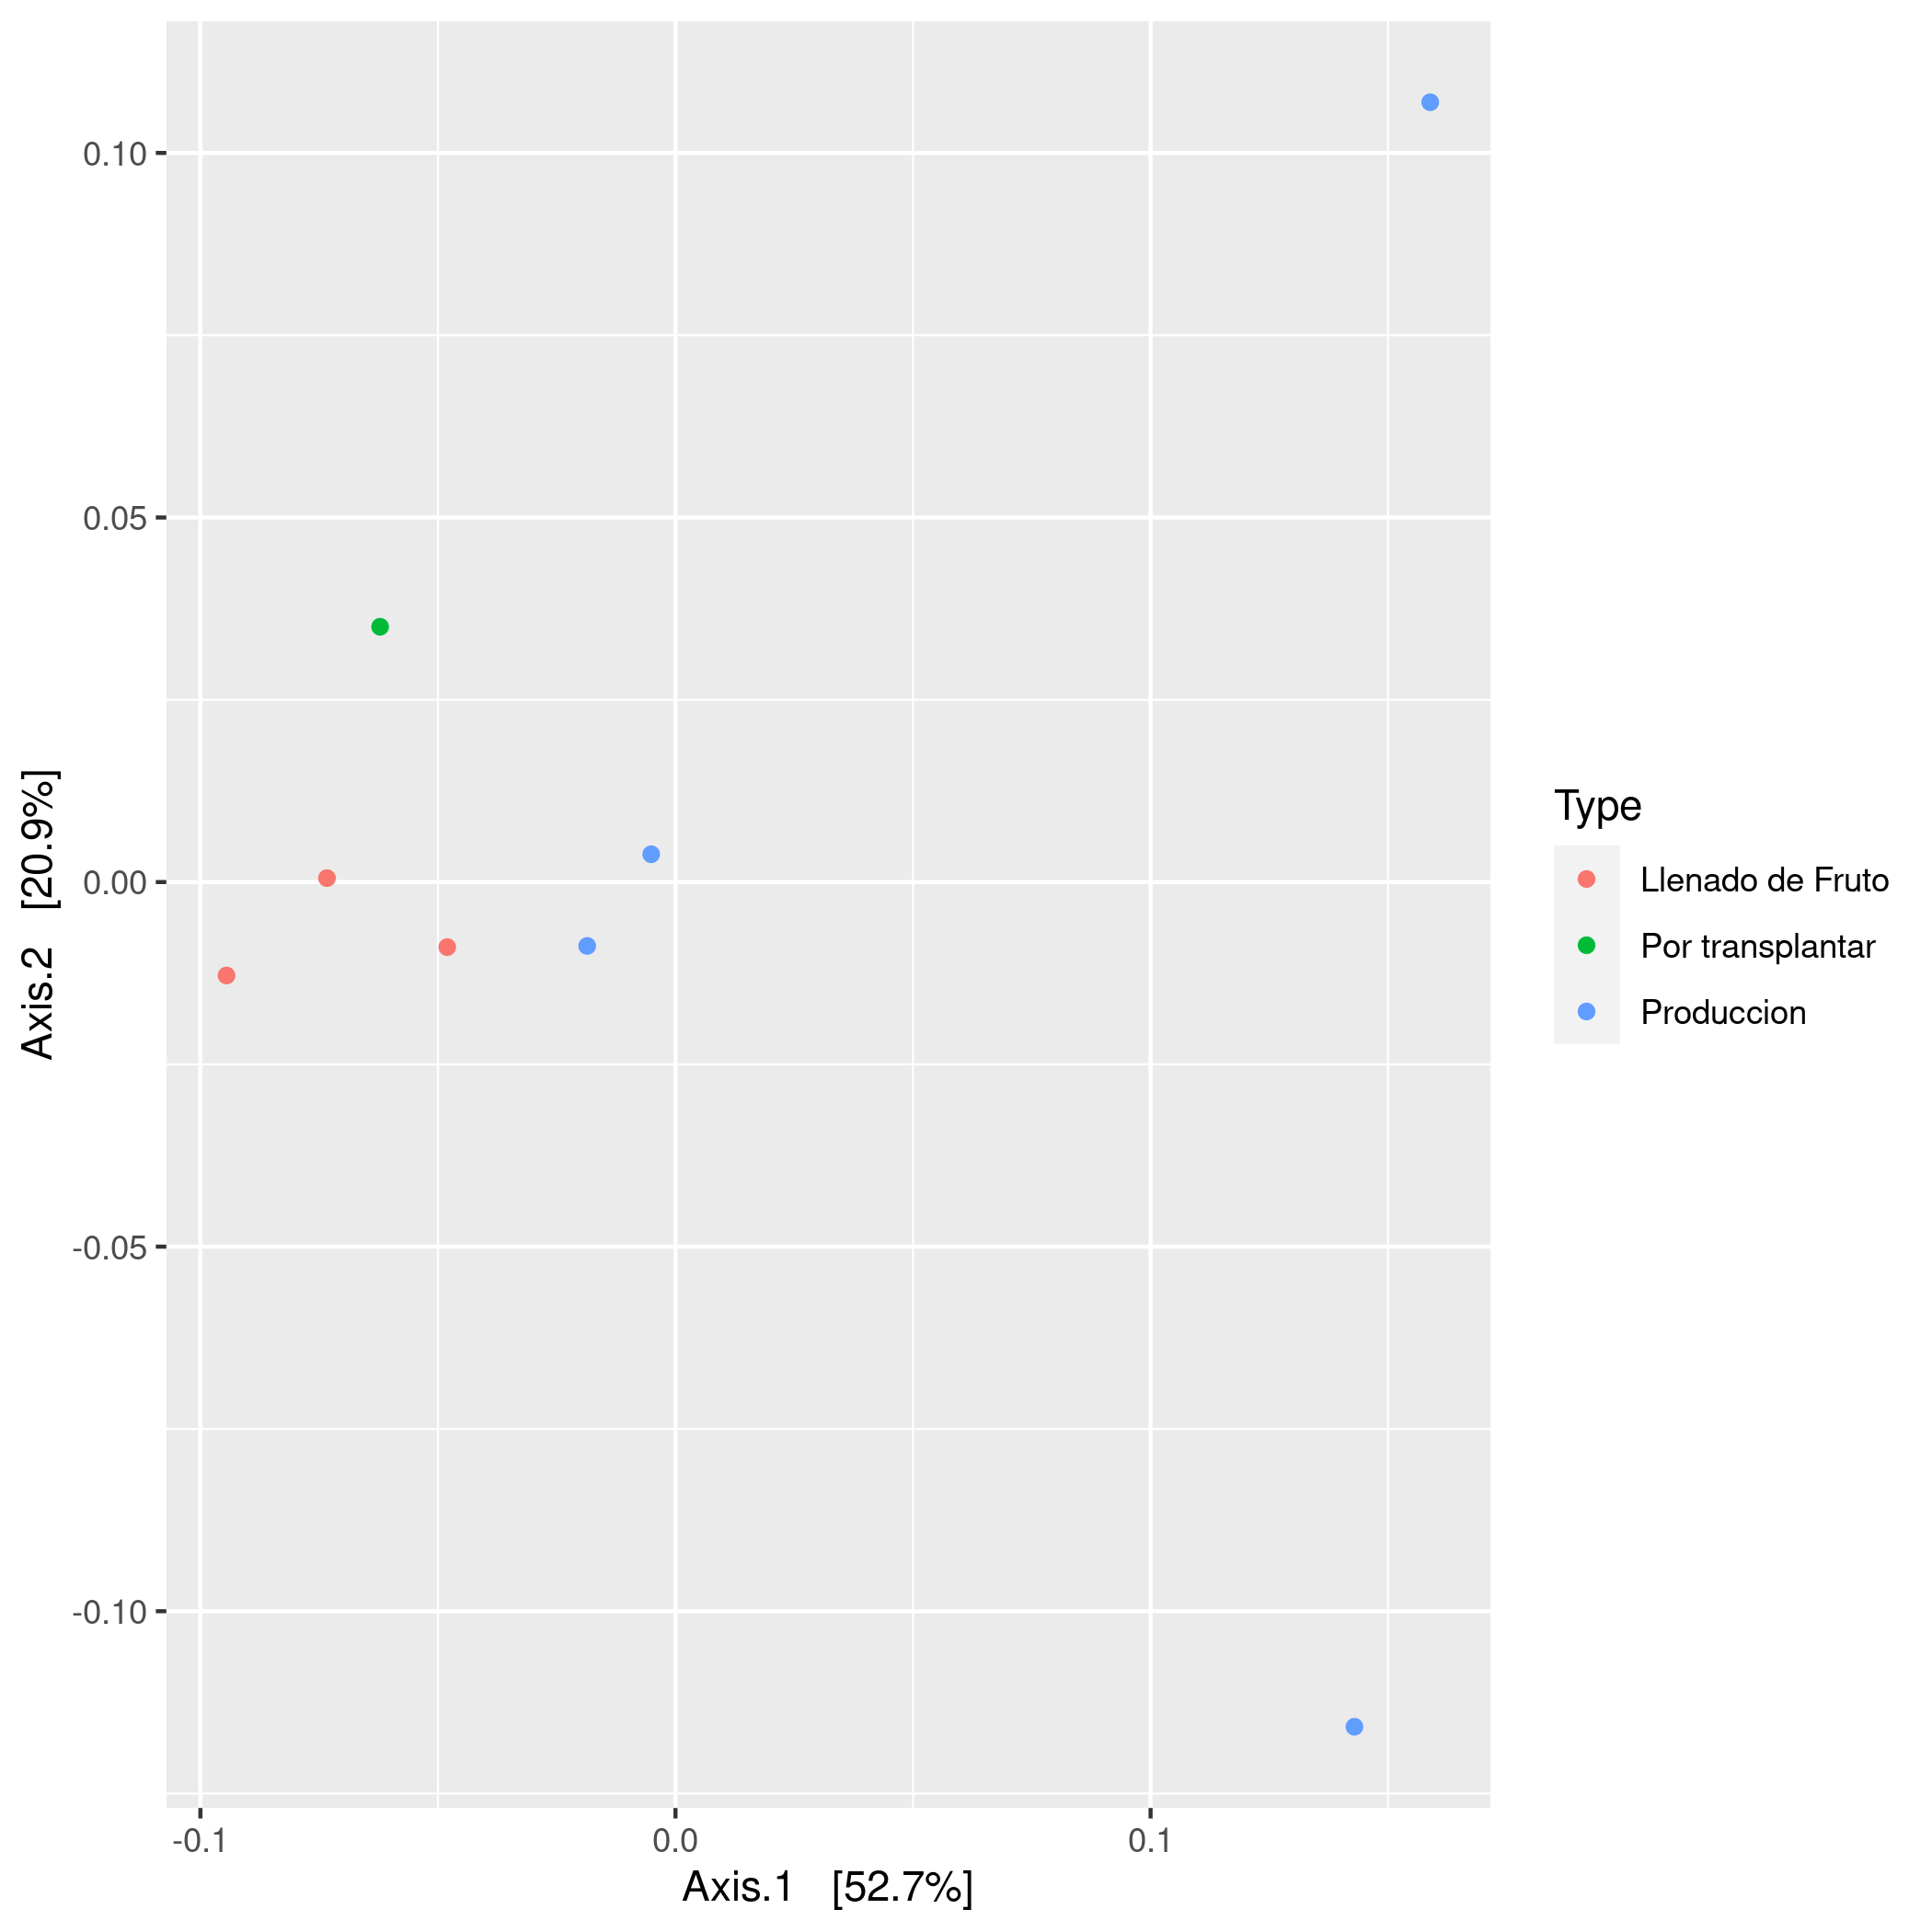
\includegraphics[scale = 0.7]{pcoa_key_otus_tomate_no_desarrollo.csv.png}
  \caption{PCoA analysis with Bray-Curtis distance of rhizosphere samples of tomate_no_desarrollo.csv, restricted to keystone OTUs.}
  \label{fig:tomate_no_desarrollo.csv_pcoa_key_otus}
\end{figure}
